\documentclass{standalone}
\usepackage{tikz}
\usetikzlibrary{patterns, positioning}


\begin{document}
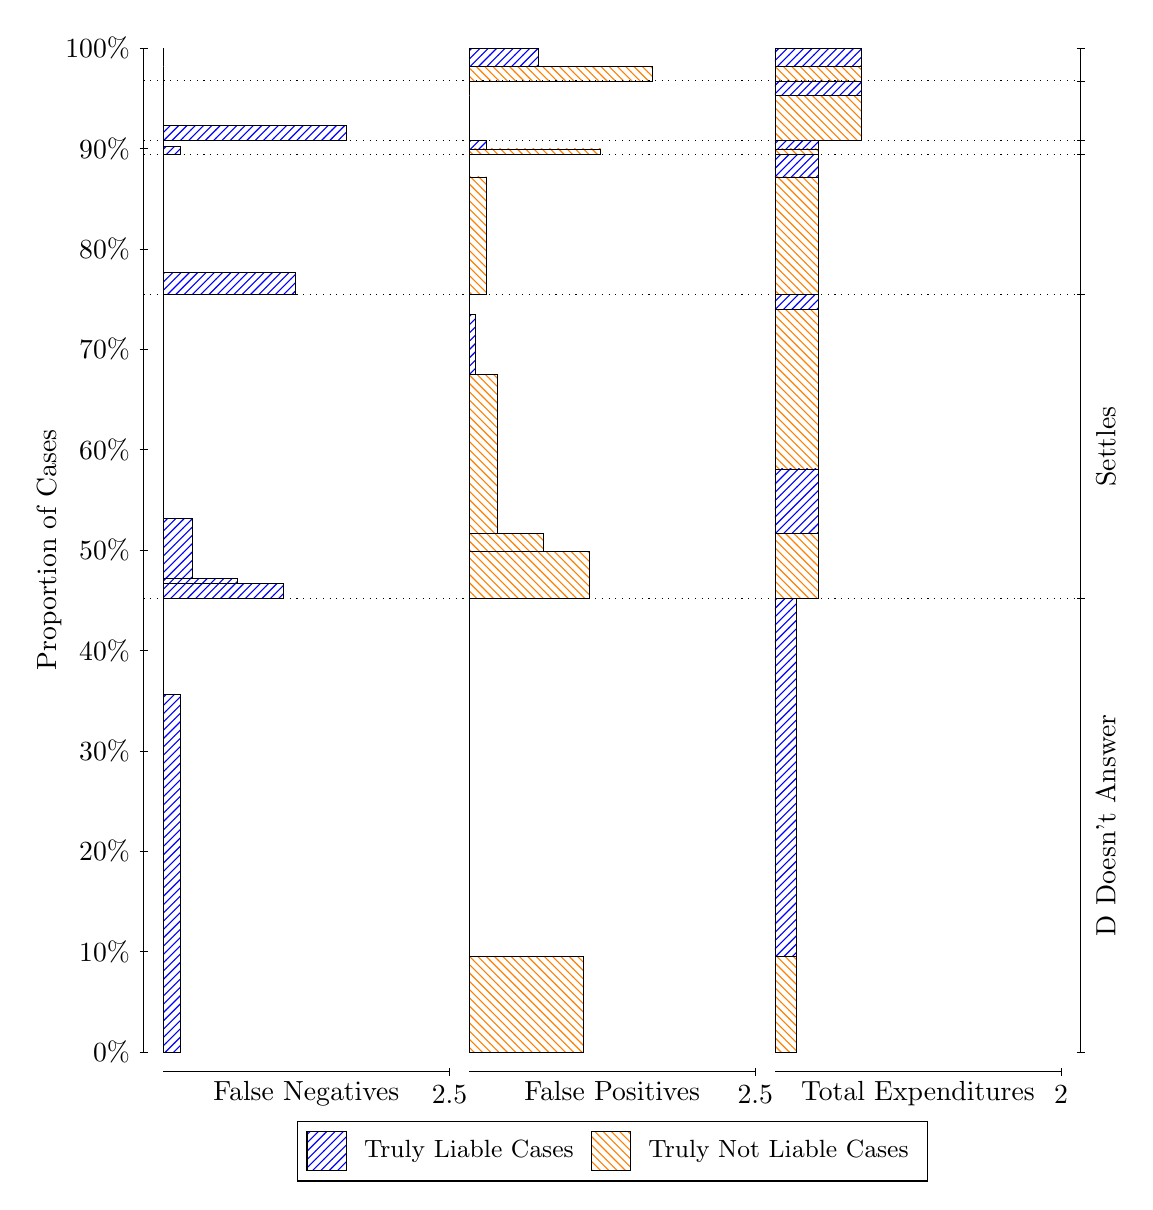
\begin{tikzpicture}
\draw[black, very thin] (1.5,1.75) -- (1.5,14.5);
\node[rotate=90, text=black, anchor=center] at (0.3, 8.125) {Proportion of Cases};
\draw[black, very thin] (1.45,1.75) -- (1.55,1.75);
\node[text=black, anchor=east] at (1.45, 1.75) {0\%};
\draw[black, very thin] (1.45,3.025) -- (1.55,3.025);
\node[text=black, anchor=east] at (1.45, 3.025) {10\%};
\draw[black, very thin] (1.45,4.3) -- (1.55,4.3);
\node[text=black, anchor=east] at (1.45, 4.3) {20\%};
\draw[black, very thin] (1.45,5.575) -- (1.55,5.575);
\node[text=black, anchor=east] at (1.45, 5.575) {30\%};
\draw[black, very thin] (1.45,6.85) -- (1.55,6.85);
\node[text=black, anchor=east] at (1.45, 6.85) {40\%};
\draw[black, very thin] (1.45,8.125) -- (1.55,8.125);
\node[text=black, anchor=east] at (1.45, 8.125) {50\%};
\draw[black, very thin] (1.45,9.4) -- (1.55,9.4);
\node[text=black, anchor=east] at (1.45, 9.4) {60\%};
\draw[black, very thin] (1.45,10.675) -- (1.55,10.675);
\node[text=black, anchor=east] at (1.45, 10.675) {70\%};
\draw[black, very thin] (1.45,11.95) -- (1.55,11.95);
\node[text=black, anchor=east] at (1.45, 11.95) {80\%};
\draw[black, very thin] (1.45,13.225) -- (1.55,13.225);
\node[text=black, anchor=east] at (1.45, 13.225) {90\%};
\draw[black, very thin] (1.45,14.5) -- (1.55,14.5);
\node[text=black, anchor=east] at (1.45, 14.5) {100\%};

\draw[black, very thin] (13.4,1.75) -- (13.4,14.5);
\draw[black, very thin] (13.35,1.75) -- (13.45,1.75);
\node[anchor=west] at (13.35, 1.75) {};
\draw[black, very thin] (13.35,7.5072) -- (13.45,7.5072);
\node[anchor=west] at (13.35, 7.5072) {};
\draw[black, very thin] (13.35,11.371) -- (13.45,11.371);
\node[anchor=west] at (13.35, 11.371) {};
\draw[black, very thin] (13.35,13.145) -- (13.45,13.145);
\node[anchor=west] at (13.35, 13.145) {};
\draw[black, very thin] (13.35,13.329) -- (13.45,13.329);
\node[anchor=west] at (13.35, 13.329) {};
\draw[black, very thin] (13.35,14.082) -- (13.45,14.082);
\node[anchor=west] at (13.35, 14.082) {};
\draw[black, very thin] (13.35,14.5) -- (13.45,14.5);
\node[anchor=west] at (13.35, 14.5) {};

\draw[black, very thin, pattern color=blue, pattern=north east lines] (1.75,1.75) rectangle (1.968,6.2942);
\draw[black, very thin, pattern color=orange, pattern=north west lines] (1.75,6.2942) rectangle (1.75,7.5072);
\draw[black, very thin, pattern color=blue, pattern=north east lines] (1.75,7.5072) rectangle (3.276,7.7025);
\draw[black, very thin, pattern color=blue, pattern=north east lines] (1.75,7.7025) rectangle (2.6947,7.7598);
\draw[black, very thin, pattern color=blue, pattern=north east lines] (1.75,7.7598) rectangle (2.1133,8.5267);
\draw[black, very thin, pattern color=orange, pattern=north west lines] (1.75,8.5267) rectangle (1.75,11.371);
\draw[black, very thin, pattern color=blue, pattern=north east lines] (1.75,11.371) rectangle (3.4213,11.653);
\draw[black, very thin, pattern color=orange, pattern=north west lines] (1.75,11.653) rectangle (1.75,13.145);
\draw[black, very thin, pattern color=blue, pattern=north east lines] (1.75,13.145) rectangle (1.968,13.255);
\draw[black, very thin, pattern color=orange, pattern=north west lines] (1.75,13.255) rectangle (1.75,13.329);
\draw[black, very thin, pattern color=blue, pattern=north east lines] (1.75,13.329) rectangle (4.0753,13.513);
\draw[black, very thin, pattern color=orange, pattern=north west lines] (1.75,13.513) rectangle (1.75,14.082);
\draw[black, very thin, pattern color=orange, pattern=north west lines] (1.75,14.082) rectangle (1.75,14.266);
\draw[black, very thin, pattern color=blue, pattern=north east lines] (1.75,14.266) rectangle (1.75,14.5);
\draw[black, very thin, pattern color=orange, pattern=north west lines] (5.6333,1.75) rectangle (7.0867,2.9629);
\draw[black, very thin, pattern color=blue, pattern=north east lines] (5.6333,2.9629) rectangle (5.6333,7.5072);
\draw[black, very thin, pattern color=orange, pattern=north west lines] (5.6333,7.5072) rectangle (7.1593,8.1038);
\draw[black, very thin, pattern color=orange, pattern=north west lines] (5.6333,8.1038) rectangle (6.578,8.3314);
\draw[black, very thin, pattern color=orange, pattern=north west lines] (5.6333,8.3314) rectangle (5.9967,10.351);
\draw[black, very thin, pattern color=blue, pattern=north east lines] (5.6333,10.351) rectangle (5.706,11.118);
\draw[black, very thin, pattern color=blue, pattern=north east lines] (5.6333,11.118) rectangle (5.6333,11.371);
\draw[black, very thin, pattern color=orange, pattern=north west lines] (5.6333,11.371) rectangle (5.8513,12.863);
\draw[black, very thin, pattern color=blue, pattern=north east lines] (5.6333,12.863) rectangle (5.6333,13.145);
\draw[black, very thin, pattern color=orange, pattern=north west lines] (5.6333,13.145) rectangle (7.3047,13.218);
\draw[black, very thin, pattern color=blue, pattern=north east lines] (5.6333,13.218) rectangle (5.8513,13.329);
\draw[black, very thin, pattern color=orange, pattern=north west lines] (5.6333,13.329) rectangle (5.6333,13.897);
\draw[black, very thin, pattern color=blue, pattern=north east lines] (5.6333,13.897) rectangle (5.6333,14.082);
\draw[black, very thin, pattern color=orange, pattern=north west lines] (5.6333,14.082) rectangle (7.9587,14.266);
\draw[black, very thin, pattern color=blue, pattern=north east lines] (5.6333,14.266) rectangle (6.5053,14.5);
\draw[black, very thin, pattern color=orange, pattern=north west lines] (9.5167,1.75) rectangle (9.7892,2.9629);
\draw[black, very thin, pattern color=blue, pattern=north east lines] (9.5167,2.9629) rectangle (9.7892,7.5072);
\draw[black, very thin, pattern color=orange, pattern=north west lines] (9.5167,7.5072) rectangle (10.062,8.3314);
\draw[black, very thin, pattern color=blue, pattern=north east lines] (9.5167,8.3314) rectangle (10.062,9.1556);
\draw[black, very thin, pattern color=orange, pattern=north west lines] (9.5167,9.1556) rectangle (10.062,11.176);
\draw[black, very thin, pattern color=blue, pattern=north east lines] (9.5167,11.176) rectangle (10.062,11.371);
\draw[black, very thin, pattern color=orange, pattern=north west lines] (9.5167,11.371) rectangle (10.062,12.863);
\draw[black, very thin, pattern color=blue, pattern=north east lines] (9.5167,12.863) rectangle (10.062,13.145);
\draw[black, very thin, pattern color=orange, pattern=north west lines] (9.5167,13.145) rectangle (10.062,13.218);
\draw[black, very thin, pattern color=blue, pattern=north east lines] (9.5167,13.218) rectangle (10.062,13.329);
\draw[black, very thin, pattern color=orange, pattern=north west lines] (9.5167,13.329) rectangle (10.607,13.897);
\draw[black, very thin, pattern color=blue, pattern=north east lines] (9.5167,13.897) rectangle (10.607,14.082);
\draw[black, very thin, pattern color=orange, pattern=north west lines] (9.5167,14.082) rectangle (10.607,14.266);
\draw[black, very thin, pattern color=blue, pattern=north east lines] (9.5167,14.266) rectangle (10.607,14.5);
\draw[black, dotted] (1.5,7.5072) -- (13.4,7.5072);
\draw[black, dotted] (1.5,11.371) -- (13.4,11.371);
\draw[black, dotted] (1.5,13.145) -- (13.4,13.145);
\draw[black, dotted] (1.5,13.329) -- (13.4,13.329);
\draw[black, dotted] (1.5,14.082) -- (13.4,14.082);
\draw[black, very thin] (1.75,1.5) -- (5.3833,1.5);
\node[text=black, anchor=north] at (3.5667, 1.5) {False Negatives};
\draw[black, very thin] (5.3833,1.45) -- (5.3833,1.55);
\node[text=black, anchor=north] at (5.3833, 1.45) {2.5};

\draw[black, very thin] (5.6333,1.5) -- (9.2667,1.5);
\node[text=black, anchor=north] at (7.45, 1.5) {False Positives};
\draw[black, very thin] (9.2667,1.45) -- (9.2667,1.55);
\node[text=black, anchor=north] at (9.2667, 1.45) {2.5};

\draw[black, very thin] (9.5167,1.5) -- (13.15,1.5);
\node[text=black, anchor=north] at (11.333, 1.5) {Total Expenditures};
\draw[black, very thin] (13.15,1.45) -- (13.15,1.55);
\node[text=black, anchor=north] at (13.15, 1.45) {2};

\node[text=black, centered, rotate=90] at (13.72, 4.6286) {D Doesn't Answer};
\node[text=black, centered, rotate=90] at (13.72, 9.439) {Settles};





\draw (7.449999999999999,1.5) node[draw=none] (baseCoordinate) {};
\begin{scope}[align=center]
        \matrix[scale=0.5, draw=black, below=0.5cm of baseCoordinate, nodes={draw}, column sep=0.1cm]{
            \node[rectangle, draw, minimum width=0.5cm, minimum height=0.5cm, pattern color=blue, pattern=north east lines] {}; &
            \node[draw=none, font=\small, text=black] (B) {Truly Liable Cases}; &
            \node[rectangle, draw, minimum width=0.5cm, minimum height=0.5cm, pattern color=orange, pattern=north west lines] {}; &
            \node[draw=none, font=\small, text=black] (B) {Truly Not Liable Cases}; \\
            };
\end{scope}

\end{tikzpicture}
\end{document}